%Chris
\section{Modellierung von Rotorblatt und Turm} \label{turm_blatt}

\subsection{Vorbetrachtung}
Die Modellierung der Rotorblätter (weiter als Blatt bezeichnet) und des Turms erfolgt analog zur Modellierung des Triebstranges. Als Grundlage für die Modellbildung dient das Feder-Masse-Dämpfer-System. Daraus soll die Bewegungs-DGL für die Blätter und des Turms abgeleitet werden. Allerdings wird hier für die Modellierung eine translatorische Bewegung betrachtet. Damit die reale Auslenkung der Blätter und des Turms modelliert wird, müssen hierzu mathematische Modelle formuliert werden, die die Dynamik des Systems in Abhängigkeit von äußeren Belastungen beschreibt. Genauer wird hier die Auslenkung infolge von außen angreifenden Kräften betrachtet. Die Verwendung eines mathematischen Ersatzmodells dient zur Vereinfachung und Überführung komplexer technischer Systeme. Dies macht das System beschreibbar und deterministisch. 
\\
Für die reale Auslenkung der Blätter und des Turms wird die Blattverbiegung als kollektiv in Windrichtung und die Turmverbiegung in Windrichtung betrachtet. Ähnlich wie beim Triebstrang haben die Systemgrößen wie Steifigkeit, Dämpfung und Masse ebenfalls eine entscheidende Rolle bei der Modellierung. Die \autoref{fig:Abbildung5.1} zeigt schematisch die Auslenkung von Blätter und Turm. Die Schubkraft \acs{FS} bewirkt dabei die Blatterverbiegung \acs{yB} und die Turmverbiegung \acs{yT}. Die Auslenkung hängt maßgeblich von der Steifigkeit und Dämpfung beider Systeme ab. Eine hohe Steifigkeit und Dämpfung führt zur einer geringeren Auslenkung und damit auch zu einem schnelleren Ausschwingen bei Belastung, während eine geringe Steifigkeit und Dämpfung zu einer höheren Auslenkung und langsameres Ausschwingen bei Belastung führt.
\begin{figure}[H]
    \centering
    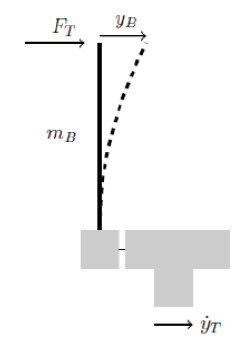
\includegraphics[scale=0.5]{Bilder/Kapitel 6/Auslenkung_Blatt.PNG}
    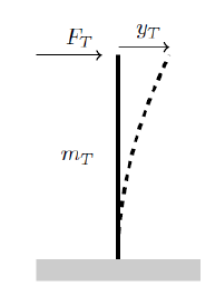
\includegraphics[scale=0.5]{Bilder/Kapitel 6/Auslenkung_Turm.PNG}
    \caption{Schematische Darstellung der Auslenkung der kollektiven Blätter \textit{(links)} und des Turms \textit{(rechts)}}
    \label{fig:Abbildung5.1}
\end{figure}
\newpage
Mit Hilfe der Bewegungs-DGL soll die reale Auslenkung der WEA beschrieben werden, damit zunächst abgeschätzt wird, ob eine Einhaltung der vorgegebenen Auslenkungsgrenzen vorliegt. Die WEA wird hierfür mit einer Bemessungswindgeschwindigkeit und einer daraus resultierenden Schubkraft \acs{FS} mechanisch von außen belastet. Das Modell wird als Funktionsblock in Matlab Simulink implementiert. 

\subsection{Feder-Masse-Dämpfer-System}
Als Grundlage für die Modellbildung dient das Feder-Masse-Dämpfer-System. Mithilfe dessen Vorüberlegungen und Ansätze wird das mathematische Modell für die Blätter und dem Turm abgeleitet. Jeder mechanische Körper besitzt eine Steifigkeit \textit{k} und eine Dämpfung \textit{d}. Sofern eine Kraft \textit{F} auf den Körper wirkt, entsteht eine Auslenkung \textit{x}, welche von der Masse \textit{m} und den vorher besagten Größen abhängt. Die \autoref{fig:Abbildung5.2}{} zeigt den grundlegenden Aufbau eines solchen Systems.
Des Weiteren entsteht an jedem Element eine sogenannte Gegenkraft, welche der einwirkenden Kraft \textit{F} entgegenwirkt. Die Summe aller Kräfte innerhalb eines Systems ergeben sich zu 0, wodurch sich folgende Kräftebilanz in \autoref{eq:Gleichung 5.1} wiederfindet. Der Zusammenhang zwischen der Auslenkung \textit{x} und der Kraft \textit{F} kann als Differentialgleichung in \autoref{eq:Gleichung 5.2} beschrieben werden.
\begin{align}
    F(t) - F_{m}(t) - F_{k}(t) - F_{d}(t) = 0 
    \label{eq:Gleichung 5.1}
\end{align}

\begin{align}
    F(t) = m \cdot \frac{\delta^2x}{\delta^2t} + d \cdot \frac{\delta x}{\delta t} + k \cdot x(t)
    \label{eq:Gleichung 5.2}
\end{align}
\begin{figure}[H]
\centering
\scalebox{0.90}{
\begin{tikzpicture}[
  scale = 1.0,thick,>=triangle 45,
  spring/.style = {decorate,decoration={zigzag,amplitude=2pt,segment length=4pt}}
  ]
  %Raster
\draw [color=gray!10] [step=1mm] (-2.5cm,-0.5cm) grid (2.5cm,-5.5cm);
\draw [color=gray!30] [step=1cm] (-2.5cm,-0.5cm) grid (2.5cm,-5.5cm);

%FederMasseDämpferSystem
	\node[coordinate] (m) at (0.0,-2.0) {};
	\node[draw,minimum size=1.5em] at (m) {$m$};
  	\draw[shorten <=16pt] (m) -- coordinate (x) ++( 2,0);
  	\draw[shorten <=16pt] (m) -- coordinate (f) ++(-2,0);
  	\draw[<-] (f) -- node[left] {$F$} ++(0,-1);
  \draw[->] (x) -- node[right] {$x$} ++(0,1);
  \draw[shorten <=9.0pt] (m) -- +(0,-.7) coordinate (c);
  \draw (c) -| +( .7,-.3) coordinate (r);
  \draw (c) -| +(-.7,-.3) coordinate (l);
  \draw (r) -| +( .2,-1) node[right,pos=.75] {$d$};
  \draw (r) -| +(-.2,-1);
  \draw (r) +(-.15,-.5) -- coordinate (d) +(.15,-.5);
  \draw[spring] (l) -- node[left] {$k$} +(0,-1);
  \draw (l) ++(0,-1) -- ++(0,-.3) coordinate (b);
  \draw (d) |- (b);
  \draw (b -| m) -- ++(0,-.5) coordinate (g);
  \draw (g) +(-.5,0) -- +(.5,0);
  \foreach \i in {-1,0,1}
    \draw (g) ++(\i*.5,0) -- ++(225:.5);
 
\end{tikzpicture}
}
\caption{Feder-Masse-Dämpfer-System}
\label{fig:Abbildung5.2}
\end{figure}
\newpage
\subsection{Modellierung}

Für die Modellierung ist zu berücksichtigen, dass die Blätter und der Turm über die Gondel mechanisch miteinander gekoppelt sind. Ähnlich wie beim Triebstrang, bei dem die low speed shaft mit dem high speed shaft über das Getriebe und dessen Übersetzungsverhältnis gekoppelt ist. Das heißt, in den jeweiligen Bewegungs-DGL haben die Auslenkung der Blätter und des Turms einen gegenseitigen Einfluss aufeinander. Der einzige Unterschied der beiden Modellansätze ist, dass beim Triebstrang aufgrund einer rotatorischen Bewegung die Torsion der Wellen betrachtet wird, wobei sich ein Verschiebungswinkel $\varphi$ ergibt und bei der Modellierung der Blätter und des Turms sich durch die translatorische Bewegung eine Auslenkung \acs{yB} und \acs{yT} ergibt, wie in \autoref{fig:Abbildung5.3} dargestellt. Die Werte zur jeweiligen Masse, Steifigkeit und Dämpfung sind bereits gegeben. Da für die gesamte Modellierung der WEA eher die Auslenkung von Bedeutung ist, gilt es die \autoref{eq:Gleichung 5.2} so umzustellen, dass die benötigte Auslenkung der Blätter und des Turms berechnet wird. Eine zu große Auslenkung würde nämlich zur Zerstörung der WEA führen und dies gilt es mit geeigneten Reglern zu begrenzen. 

\begin{figure}[H]
\centering
\scalebox{0.90}{
\begin{tikzpicture}[
  scale = 1.0,thick,>=triangle 45,
  spring/.style = {decorate,decoration={zigzag,amplitude=2pt,segment length=4pt}}
  ]
  %Raster
\draw [color=gray!10] [step=1mm] (-2.5cm,1.1cm) grid (2.5cm,-7.5cm);
\draw [color=gray!30] [step=1cm] (-2.5cm,1.1cm) grid (2.5cm,-7.5cm);

%Blattmodell
  \node[draw,minimum size=1.5em] (mB) {$3\cdot m_B$};
  \draw[shorten <=3pt] (mB) -- coordinate (yB) ++( 2,0);
  \draw[shorten <=3pt] (mB) -- coordinate (f) ++(-2,0);
  \draw[<-] (f) -- node[left] {$F_S(t)$} ++(0,-1);
  \draw[->] (yB) -- node[right] {$y_B(t)$} ++(0,1);
  \draw (mB) -- +(0,-.7) coordinate (cB);
  \draw (cB) -| +( .7,-.3) coordinate (rB);
  \draw (cB) -| +(-.7,-.3) coordinate (lB);
  \draw (rB) -| +( .2,-1) node[right,pos=.75] {$3\cdot d_B$};
  \draw (rB) -| +(-.2,-1);
  \draw (rB) +(-.15,-.5) -- coordinate (dB) +(.15,-.5);
  \draw[spring] (lB) -- node[left] {$3\cdot k_B$} +(0,-1);
  \draw (lB) ++(0,-1) -- ++(0,-.3) coordinate (bB);
  \draw (dB) |- (bB);
  \draw (bB -| mB) -- ++(0,-.5) coordinate (gB);

%Turmmodell
	\node[coordinate] (mT) at (0.0,-4.0) {};
	\draw[shorten <=9pt] (mT) -- (gB);
	\node[draw,minimum size=1.5em] at (mT) {$m_T$};
  	\draw[shorten <=16pt] (mT) -- coordinate (yT) ++( 2,0);
  	\draw[shorten <=16pt] (mT) -- coordinate (f) ++(-2,0);
  	\draw[<-] (f) -- node[left] {$F_S(t)$} ++(0,-1);
  \draw[->] (yT) -- node[right] {$y_T(t)$} ++(0,1);
  \draw[shorten <=9.0pt] (mT) -- +(0,-.7) coordinate (c);
  \draw (c) -| +( .7,-.3) coordinate (r);
  \draw (c) -| +(-.7,-.3) coordinate (l);
  \draw (r) -| +( .2,-1) node[right,pos=.75] {$d_T$};
  \draw (r) -| +(-.2,-1);
  \draw (r) +(-.15,-.5) -- coordinate (d) +(.15,-.5);
  \draw[spring] (l) -- node[left] {$k_T$} +(0,-1);
  \draw (l) ++(0,-1) -- ++(0,-.3) coordinate (b);
  \draw (d) |- (b);
  \draw (b -| mT) -- ++(0,-.5) coordinate (g);
  \draw (g) +(-.5,0) -- +(.5,0);
  \foreach \i in {-1,0,1}
    \draw (g) ++(\i*.5,0) -- ++(225:.5);
 
\end{tikzpicture}
}
\caption{Modell des Turms und der Blätter}
\label{fig:Abbildung5.3}
\end{figure}
\newpage
Die Auslenkung der kollektiven Blätter wirkt der Auslenkung des Turms entgegen, wodurch die Gegenkräfte der Steifigkeit und Dämpfung der Blätter mit einem positiven Vorzeichen in die Bewegungs-DGL mit einfließen. Die eigentliche Auslenkung ergibt sich aufgrund der mechanischen Kopplung aus der Differenz zwischen Blattverbiegung \acs{yB} und Turmverbiegung \acs{yT}. Die Steifigkeit und Dämpfung beziehen sich lediglich auf ein Blatt, wodurch diese Faktoren mit 3 multipliziert werden, um insgesamt das Verhalten der drei Blätter abzubilden.



Damit ergibt sich für die Bewegungs-DGL des Turms:

\begin{align}\label{eq:Gleichung 6.3}
    \boxed{\ddot{\acs{yT}}=\frac{-\acs{kT} \cdot \acs{yT}- \acs{dT} \cdot \dot{\acs{yT}}+ 3 \cdot \acs{kB} \cdot(\acs{yB}-\acs{yT})+ 3\cdot \acs{dB} \cdot (\dot{\acs{yB}}-\dot{\acs{yT}})+\acs{FS}} {\acs{mT}}}
\end{align}

Gleiches gilt für die effektiv schwingende Blattmasse \acs{mB}. Aufgrund dessen verringert sich die Schubkraft \acs{FS} um Eindrittel. Für die Blätter ergibt sich folgende Bewegungs-DGL:

\begin{align}\label{eq:Gleichung6.4}
    \boxed{\ddot{\acs{yB}}=\frac{-3 \cdot \acs{kB} \cdot(\acs{yB}-\acs{yT})-3 \cdot \acs{dB} \cdot (\dot{\acs{yB}}-\dot{\acs{yT}})+\acs{FS}} {3\cdot\acs{mB}}}
\end{align}

\subsection{Simulationsergebnisse}
Zu Beginn des Kapitels wurde bereits erwähnt, dass das Modell zu Blätter und Turm in einem Funktionsblock in Matlab Simulink implementiert wird. Zur vorläufigen Überprüfung des Modells wird vorerst das System mit einer konstanten Schubkraft \acs{FS} im Bemessungsbetrieb belastet. Dies soll zunächst eine Auskunft darüber geben, ob die resultierende Auslenkung den Erwartungen entsprechen. Um eine genaue Aussage über das korrekte Verhalten des Modells zu treffen, muss das gesamte Modell mit Regelung betrachtet und getestet werden. 
Die Bemessungswindleistung der WEA beträgt:
\begin{align}
    \acs{v1} = 10 \frac {m}{s}
\end{align}
\\
Es wird ein Schubkraftbeiwert von \acs{cT} = 0,8 angenommen. Der Schubkraftbeiwert \acs{cT} sowie die daraus resultierende Schubkraft \acs{FS} ergibt sich später aus dem Kennfeld der WEA. Mithilfe der \autoref{eq:Gleichung6.4} lässt sich nun eine Schubkraft \acs{FS} berechnen, die das System belasten soll. Die restlichen benötigten Größen sind Konstanten und bereits gegeben. Das Ergebnis ist der \autoref{eq:Gleichung 6.7} zu entnehmen. Die \autoref{fig:Abbildung5.4} zeigt die Ein- und Ausgangsparameter des Modells in Blockdarstellung für die Simulation.
\\
\begin{align}
    \acs{FS} &= \frac{1}{2} \cdot \rho \cdot \pi \cdot \acs{R}^2 \cdot \acs{cT} \cdot \acs{v1}^2 \label{eq:Gleichung6.6} \\
    \acs{FS} &= \frac{1}{2} \cdot 1,225 \frac{kg}{m^3} \cdot \pi \cdot (63m)^2 \cdot 0,8 \cdot (10 \frac{m}{s})^2 \nonumber \\
    \acs{FS} &= \underline{\underline{610980,1 N}} \label{eq:Gleichung 6.7}
\end{align}

\begin{figure}[H]
   \centering
   \begin{pspicture}[showgrid=false](0,0)(10,5)
        \psframe(0,0)(10,5)
        % Eingänge
        \psline{->}(1,2.5)(3.5,2.5)
        \rput(1,2.9){\footnotesize \acs{FS}}

        % Modell
        \psframe[linecolor=black,fillcolor=lightGrey,fillstyle=solid](3.5,0.5)(6.5,4.5)
        \rput(5,2.8){\small Blatt- und}
        \rput(5,2.3){\small Turmmodell}
        % Ausgänge
        \psline{->}(6.5,3.0)(9,3.0)
        \rput(9,3.4){\footnotesize \acs{yT}}
        \psline{->}(6.5,2.0)(9,2.0)
        \rput(9,2.4){\footnotesize \acs{yB}}
    \end{pspicture}
   \caption[Übersicht Blatt- und Turmmodell]{Blockdarstellung des Blatt- und Turmmodells inklusive der Ein- und Ausgangsparameter}
   \label{fig:Abbildung5.4}
\end{figure}

Mit dem Ergebnis aus \autoref{eq:Gleichung 6.7} wird nun das Modell von außen mit einer konstanten Schubkraft \acs{FS} belastet. Die \autoref{fig:Abbildung5.5} zeigt die Auslenkungen von den kollektiven Blättern und des Turms. Aus der Simulation ist zu erkennen, dass die Auslenkung der Blätter deutlich höher im Vergleich zur Auslenkung des Turms ist. Dies begründet sich dadurch, dass der Turm eine deutlich größere Steifigkeit und Dämpfung aufweist. Zu Beginn der Belastung ist ein deutliches Schwingen beider Systeme zu erkennen. Nach einer gewissen Zeit erreichen Blätter und Turm einen stationären Endwert, wobei der Turm etwas früher einen stationären Endwert erreicht. Das Ausmaß der Auslenkung von Blätter und Turm wird in Bezug auf die vorgegebenen Grenzen so weit eingehalten. Jedoch muss dies im Gesamtmodell erneut verifiziert werden.
\\
Zusammenfassend lässt sich sagen, dass das Simulationsergebnis zu den Blättern und dem Turm den Erwartungen entspricht. Für eine genauere Aussage zur Richtigkeit der Modelle ist die Gesamtheit der Modellierung und dessen Ergebnis zu betrachten und neu zu beurteilen. Hier wurde lediglich die WEA mit dessen Bemessungswindleistung belastet. Im Realfall sind deutlich höhere Windgeschwindigkeiten durchaus denkbar. Des Weiteren geht die Windgeschwindigkeit quadratisch in die \autoref{eq:Gleichung6.6} mit ein, so dass die Schubkraft \acs{FS} ebenfalls quadratisch mit der Windgeschwindigkeit steigt und damit die WEA deutlich mehr belastet wird, was widerrum eine höhere Auslenkung beider Systeme zur Folge hat. Durch geeignete Pitchverstellung lässt sich jedoch die Belastung der WEA bei steigender Schubkraft \acs{FS} verringern, wodurch die erzeugte Energie zwar verringert wird, aber damit wird die WEA nicht durch zu hohe Belastungen zerstört. 

 \begin{figure}[H]
    \centering
    \fbox{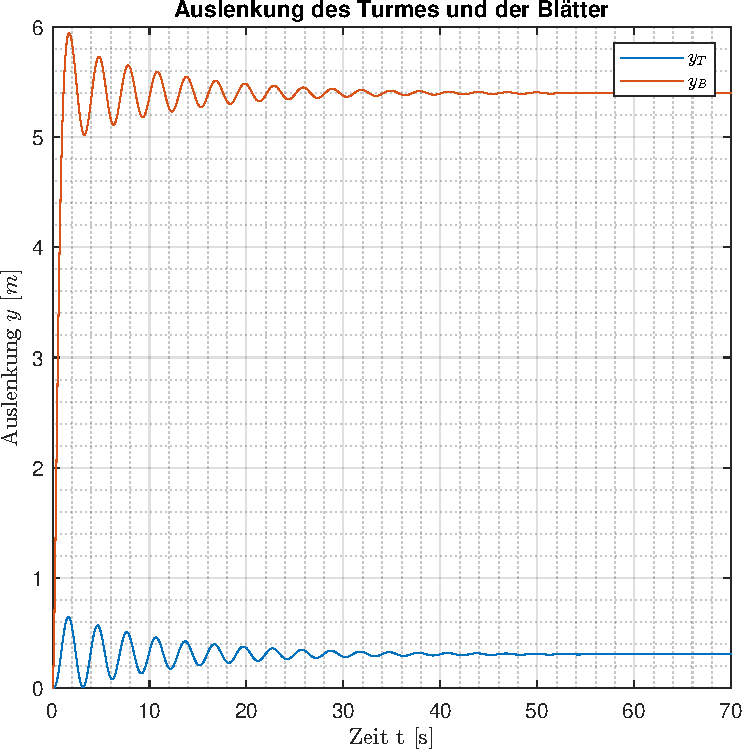
\includegraphics[width=0.9\textwidth]{Bilder/Kapitel 6/Auslenkungen.pdf}}
    \caption[Turm- und Blattauslenkung]{Auslenkung der kollektiven Blätter \textit{(orange)} und des Turmes \textit{(blau)}}
    \label{fig:Abbildung5.5}
\end{figure}

 %\underline{}
 
 %\underline{\underline{}}
 
 